\subsection{Especificación del Plan de Pruebas}
Se realizarán cuatro tipos de pruebas para garantizar la calidad del sistema: pruebas unitarias, pruebas de integración, pruebas de usabilidad y pruebas de accesibilidad.
\subsubsection{Pruebas Unitarias}
Las pruebas unitarias se realizarán para comprobar que cada componente del sistema funciona correctamente de forma aislada.
Para ello, se utilizará el framework de pruebas Jest tanto para el subsistema \textbf{restapi} como para el subsistema \textbf{webapp}.
\begin{itemize}
    \item \textbf{Pruebas Unitarias restapi}: Se realizarán pruebas unitarias para cada \textit{router} del subsistema \textbf{restapi}, de esta manera se comprueba que las rutas de la API REST funcionan correctamente.
    \item \textbf{Pruebas Unitarias webapp}: Se realizarán pruebas unitarias para los componentes más imporantes del subsistema \textbf{webapp} para comprobar que se renderizan correctamente.
\end{itemize}

\subsubsection{Pruebas de Integración}
Las pruebas de integración se realizarán para comprobar que los distintos componentes del sistema funcionan correctamente en conjunto.
Se realizarán en el subsistema \textbf{webapp}. Estas pruebas reciben el nombre de pruebas \textit{end-to-end} y se realizarán con el framework de 
pruebas jest-cucumber y Puppeteer, que permite simular la interacción de un usuario con la aplicación y son muy descriptivas al iincluir escenarios de prueba escritos en lenguaje natural.

\subsubsection{Pruebas de Usabilidad}
Las pruebas de usabilidad se realizarán para comprobar que la interfaz de usuario es intuitiva y fácil de usar.
Se realizarán pruebas de usabilidad en el subsistema \textbf{webapp} con usuarios reales, que evaluarán la interfaz de usuario y proporcionarán retroalimentación sobre su usabilidad.
Por cuestiones de tiempo, estas pruebas se realizarán con un grupo reducido de usuarios.

\subsubsection{Pruebas de Accesibilidad}
Las pruebas de accesibilidad se realizarán para comprobar que la aplicación es accesible para personas con discapacidades.
Se utilizará la herramienta de evaluación de accesibilidad de Google Lighthouse y WAVE para comprobar que la aplicación cumple con los estándares de accesibilidad.


\subsubsection{Especificación técnica del Plan de Pruebas}
En esta sección se detallará como se llevarán a cabo las pruebas de cada tipo y se especificarán los criterios de aceptación para cada una de ellas.
Además, se especifica el dispositivo y navegador en el que se realizarán las pruebas.

\subsubsubsection{Dispositivo y navegador para las pruebas}
Las pruebas se realizarán en un ordenador portátil con las siguientes características:
\begin{itemize}
    \item \textbf{Sistema Operativo}: macOS Sonoma 14.5.
    \item \textbf{Procesador}: Apple M3 Pro Max.
    \item \textbf{CPU}: 14 núcleos.
    \item \textbf{GPU}: 30 núcleos.
    \item \textbf{Memoria RAM}: 36 GB.
\end{itemize}

Como navegador se utilizará Google Chrome en su última versión para las pruebas unitarias y de integración.
Para el resto de pruebas se utilizará Google Chrome, Mozilla Firefox y Safari.
Las versiones de los navegadores son las siguientes:
\begin{itemize}
    \item \textbf{Google Chrome}: Versión 126.0.6478.127 (64 bits).
    \item \textbf{Mozilla Firefox}: Versión 127.0.2 (64 bits).
    \item \textbf{Safari}: Versión 17.5 (19618.2.12.11.6)
\end{itemize}

\subsubsubsection{Entorno de pruebas y datos de prueba}
Las pruebas unitarias se realizarán en un entorno de test local, se han creado datos de prueba que simulan la información que se almacenará en la base de datos y se usa una base de datos de pruebas.
Para las pruebas de integración se utilizarán datos reales de la base de datos de desarrollo y se simularán las interacciones de los usuarios, para ello se ejecutarán los tests en un entorno de local de desarrollo.
Para las pruebas de usabilidad y accesibilidad se utilizará un entorno de producción, ya que se necesitan datos reales y usuarios reales para evaluar la usabilidad y accesibilidad de la aplicación.


\subsection{Resultados de las Pruebas}
En esta sección se mostrarán los resultados de las pruebas realizadas y se analizarán los resultados obtenidos.

\subsubsection{Pruebas Unitarias}
Las pruebas unitarias se han realizado con éxito, se han comprobado que los componentes del sistema funcionan correctamente de forma aislada.
Se han realizado pruebas unitarias para cada \textit{router} del subsistema \textbf{restapi} y para los componentes más importantes del subsistema \textbf{webapp}. 

En el subsistema \textbf{restapi} se han realizado 51 pruebas unitarias, todas ellas han pasado con éxito obteniendo un 76.78\% de cobertura de código para \textit{routers}.
Se puede ver detallado el porcentaje de cobertura de código en la \coloredUnderline{\hyperlink{fig:6_8_Cobertura-Code-Restapi}{Figura \ref*{fig:6_8_Cobertura-Code-Restapi}: \nameref*{fig:6_8_Cobertura-Code-Restapi}}}.
\begin{figure}[H]
    \hypertarget{fig:6_8_Cobertura-Code-Restapi}{}
    \centering
    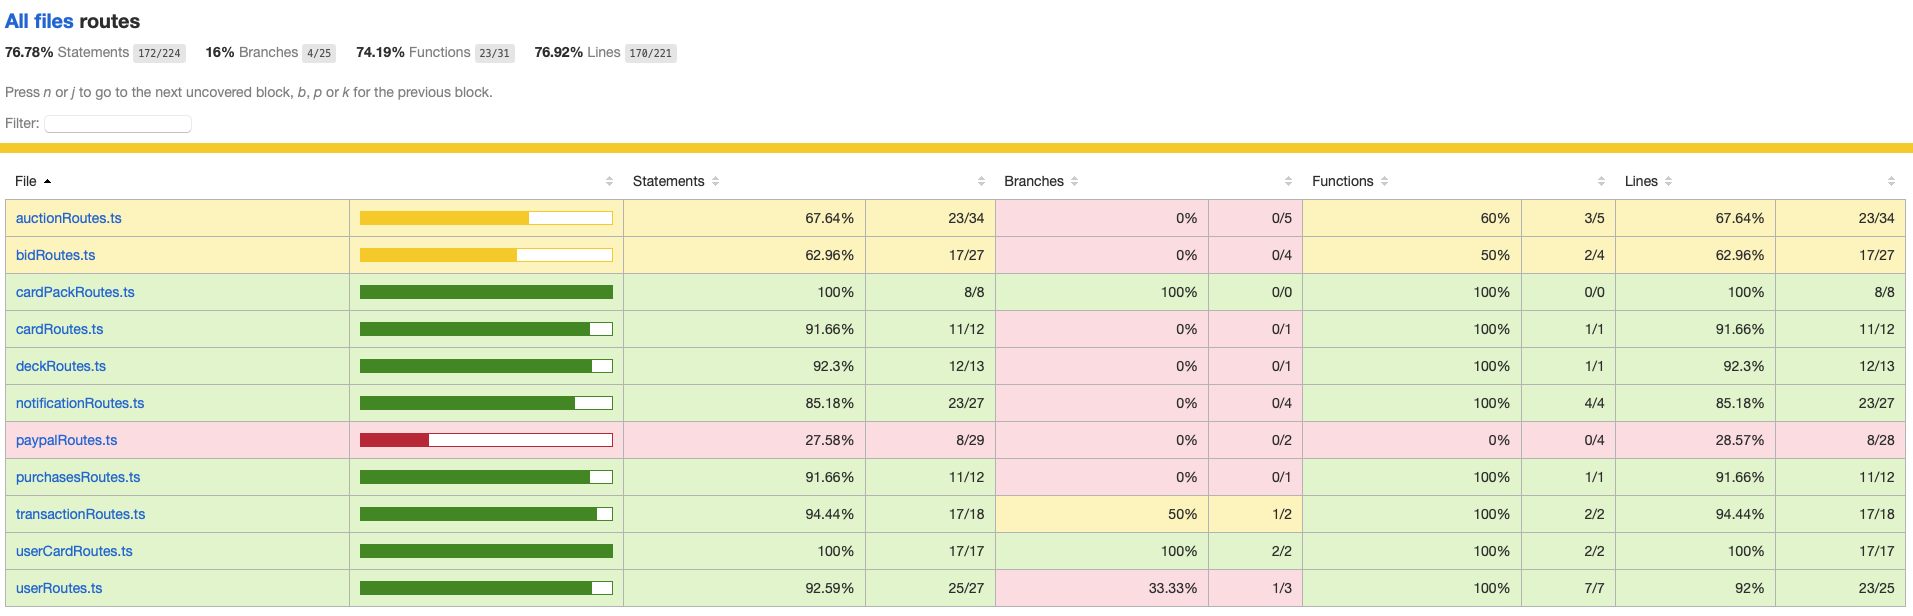
\includegraphics[width=0.8\linewidth]{figures/6-Analisis/6-Pruebas/6_8-Coverage-Restapi.png}
    \caption{Cobertura de Código del Subsistema restapi}
    \label{fig:6_8_Cobertura-Code-Restapi}
\end{figure}

En el subsistema \textbf{webapp} se han realizado 5 pruebas unitarias automáticas, se han probado los componentes más importantes de la aplicación y todas han pasado con éxito.
El resto de componentes se han probado de forma manual y se ha comprobado que su comportamiento es el esperado.


\subsubsection{Pruebas de Integración}
Las pruebas de integración se han realizado con éxito, se han comprobado que los distintos componentes del sistema funcionan correctamente en conjunto.
Se han realizado pruebas de integración en el subsistema \textbf{webapp} con el framework jest-cucumber y Puppeteer.
Se han realizado 3 pruebas de integración automáticas, todas ellas han pasado con éxito.
Las pruebas que se han realizado son las siguientes:
\begin{itemize}
    \item \textbf{Prueba de Inicio de Sesión Exitoso}: Se ha comprobado que el inicio de sesión funciona correctamente. De esta forma, se ha comprobado que el usuario puede iniciar sesión con sus credenciales y acceder a la aplicación, 
    lo que significa que la conexión con el backend funciona correctamente y la integración de los componentes de la aplicación es correcta.
    \item \textbf{Prueba de Inicio de Sesión Fallido}: Se ha comprobado que el inicio de sesión falla cuando las credenciales son incorrectas. De esta forma, se ha comprobado que la aplicación responde correctamente a errores en el inicio de sesión.
     \item \textbf{Prueba de Registro de Usuario Fallido}: Se ha comprobado que el registro de usuario falla cuando los datos introducidos no son válidos. 
     Se verifica que la aplicación responde correctamente a errores en el registro de usuario y se resaltan los campos con errores.
\end{itemize}

El resto de pruebas de integración se han realizado de forma manual y se ha comprobado que el comportamiento de la aplicación es el esperado.

\subsubsection{Pruebas de Usabilidad}
Se ha creado un formulario de evaluación de usabilidad que se les ha proporcionado a los usuarios para que evalúen la interfaz de usuario.
Se han realizado pruebas de usabilidad con 3 usuarios reales, que han evaluado la interfaz de usuario y han proporcionado retroalimentación sobre su usabilidad.
Estos usuarios, que no han participado en el desarrollo de la aplicación, han tenido que completar una serie de tareas y responder a preguntas sobre la usabilidad de la aplicación.
Los usuarios tienen una experiencia variada en el uso de aplicaciones web y representan a los diferentes tipos de usuarios que utilizarán la aplicación.
Los datos de los usuarios son los siguientes:
\begin{itemize}
    \item \textbf{Usuario 1}: Hombre de 51 años, con poca experiencia en el uso de aplicaciones web. No ha utilizado aplicaciones similares anteriormente ni realizado compras en línea.
    \item \textbf{Usuario 2}: Mujer de 22 años, con mucha experiencia en el uso de aplicaciones web. Ha utilizado aplicaciones similares anteriormente y ha realizado compras en línea.
    \item \textbf{Usuario 3}: Mujer de 18 años, con experiencia en el uso de aplicaciones web. Ha utilizado aplicaciones similares anteriormente, pero no ha llegado a realizar compras en ellas.
\end{itemize}

Se les ha trasladado el siguiente cuestionario para evaluar la usabilidad de la aplicación:
\begin{itemize}
    \item \textbf{Facilidad de Uso}: ¿Cómo de fácil ha sido para ti utilizar la aplicación?
    \item \textbf{Claridad de la Información}: ¿La información presentada en la aplicación ha sido clara y fácil de entender?
    \item \textbf{Diseño de la Interfaz}: ¿Qué opinas del diseño de la interfaz de usuario?
    \item \textbf{Facilidad de Navegación}: ¿Has encontrado fácilmente lo que buscabas en la aplicación?
    \item \textbf{Satisfacción General}: ¿Qué opinas de la aplicación en general?
